\documentclass{standalone}
\usepackage{tikz}
\usetikzlibrary{calc}           % 坐标插值、垂足等
\usetikzlibrary{angles, quotes} % 角度标注
\usetikzlibrary{arrows.meta}    % 箭头样式

\begin{document}

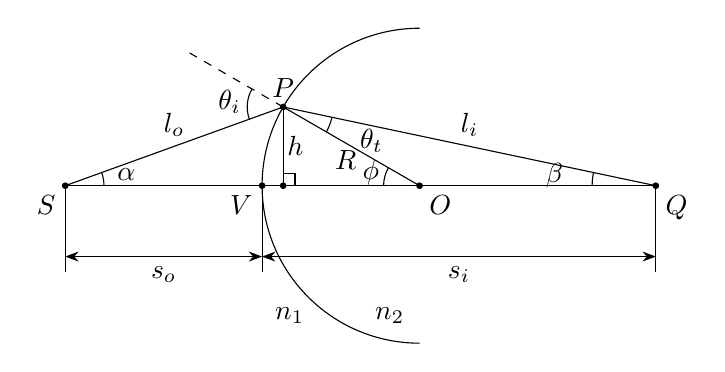
\begin{tikzpicture}[]

    % 定义关键坐标
    \coordinate (O) at (2, 0);                      % 圆心
    \coordinate (V) at (0, 0);                      % 顶点
    \coordinate (S) at (-2.5, 0);                   % 左焦点
    \coordinate (P) at ($(O) + (150:2)$);           % 交点
    \coordinate (Q) at (5, 0);                      % 右焦点
    % 绘图辅助坐标
    \coordinate (P_out) at ($(O) + (150:3.4)$);     % 交点延长线
    \coordinate (P_perp) at (P |- O);               % 垂点
    \coordinate (S_below) at ($(S) + (0, -0.9)$);
    \coordinate (V_below) at ($(V) + (0, -0.9)$);
    \coordinate (Q_below) at ($(Q) + (0, -0.9)$);


    % 画左半圆
    \draw (O) ++(90:2) arc (90:270:2);
    % 连线 SQ, SP, PQ, OP
    \draw (S) -- (Q);
    \draw (S) -- (P) node[midway, above] {$l_o$};
    \draw (P) -- (Q) node[midway, above] {$l_i$};
    \draw (O) -- (P) node[midway, below, xshift=-2pt, yshift=2pt] {$R$};
    \draw[dashed] (P) -- (P_out);   % 延长 OP
    % 画高
    \draw (P) -- (P_perp) node[midway, right, xshift=-2pt] {$h$};
    \draw (P_perp) ++(0.15,0) |- ++(-0.15,0.15);
    % 折射角 θ_t
    \pic [draw, "$\theta_t$", angle radius=18pt, angle eccentricity=1.9]
        {angle=O--P--Q};
    % 入射角 θ_i
    \pic [draw, "$\theta_i$", angle radius=13pt, angle eccentricity=1.5]
        {angle=P_out--P--S};
    % ∠OSP = α，∠POS = φ，∠PQO = β
    \pic [draw, "$\alpha$", angle radius=14pt, angle eccentricity=1.6]
        {angle=O--S--P};
    \pic [draw, "$\phi$", angle radius=13pt, angle eccentricity=1.4]
        {angle=P--O--S};
    \pic [draw, "$\beta$", angle radius=23pt, angle eccentricity=1.6]
        {angle=P--Q--O};
    % 画点
    \filldraw (O) circle (1pt) node[below right] {$O$};
    \filldraw (V) circle (1pt) node[below left]  {$V$};
    \filldraw (S) circle (1pt) node[below left] {$S$};
    \filldraw (P) circle (1pt) node[above]  {$P$};
    \filldraw (P_perp) circle (1pt);
    \filldraw (Q) circle (1pt) node[below right]  {$Q$};
    % 画 s_o 和 s_i，并标记折射率
    \draw (S) -- ($(S_below) + (0, -0.2)$);
    \draw (V) -- ($(V_below) + (0, -0.2)$);
    \draw (Q) -- ($(Q_below) + (0, -0.2)$);
    \draw[<->, >=Stealth] (S_below) -- (V_below) 
        node[midway, below] {$s_o$} 
        node [right, below, xshift=10pt, yshift=-15pt] {$n_1$};
    \draw[<->, >=Stealth] (V_below) -- (Q_below) 
        node[midway, below] {$s_i$} 
        node [midway, below, xshift=-25pt, yshift=-15pt] {$n_2$};
    

\end{tikzpicture}

\end{document}
